\documentclass[12pt,letterpaper]{article}
\usepackage{graphicx,textcomp}
\usepackage{natbib}
\usepackage{setspace}
\usepackage{fullpage}
\usepackage{color}
\usepackage[reqno]{amsmath}
\usepackage{amsthm}
\usepackage{fancyvrb}
\usepackage{amssymb,enumerate}
\usepackage[all]{xy}
\usepackage{endnotes}
\usepackage{lscape}
\newtheorem{com}{Comment}
\usepackage{float}
\usepackage{hyperref}
\newtheorem{lem} {Lemma}
\newtheorem{prop}{Proposition}
\newtheorem{thm}{Theorem}
\newtheorem{defn}{Definition}
\newtheorem{cor}{Corollary}
\newtheorem{obs}{Observation}
\usepackage[compact]{titlesec}
\usepackage{dcolumn}
\usepackage{tikz}
\usetikzlibrary{arrows}
\usepackage{multirow}
\usepackage{xcolor}
\newcolumntype{.}{D{.}{.}{-1}}
\newcolumntype{d}[1]{D{.}{.}{#1}}
\definecolor{light-gray}{gray}{0.65}
\usepackage{url}
\usepackage{listings}
\usepackage{color}

\definecolor{codegreen}{rgb}{0,0.6,0}
\definecolor{codegray}{rgb}{0.5,0.5,0.5}
\definecolor{codepurple}{rgb}{0.58,0,0.82}
\definecolor{backcolour}{rgb}{0.95,0.95,0.92}

\lstdefinestyle{mystyle}{
	backgroundcolor=\color{backcolour},   
	commentstyle=\color{codegreen},
	keywordstyle=\color{magenta},
	numberstyle=\tiny\color{codegray},
	stringstyle=\color{codepurple},
	basicstyle=\footnotesize,
	breakatwhitespace=false,         
	breaklines=true,                 
	captionpos=b,                    
	keepspaces=true,                 
	numbers=left,                    
	numbersep=5pt,                  
	showspaces=false,                
	showstringspaces=false,
	showtabs=false,                  
	tabsize=2
}
\lstset{style=mystyle}
\newcommand{\Sref}[1]{Section~\ref{#1}}
\newtheorem{hyp}{Hypothesis}

\title{Problem Set 2}
\date{Due: October 15, 2023}
\author{Applied Stats/Quant Methods 1}

\begin{document}
	\maketitle
	\section*{Instructions}
\begin{itemize}
	\item Please show your work! You may lose points by simply writing in the answer. If the problem requires you to execute commands in \texttt{R}, please include the code you used to get your answers. Please also include the \texttt{.R} file that contains your code. If you are not sure if work needs to be shown for a particular problem, please ask.
	\item Your homework should be submitted electronically on GitHub.
	\item This problem set is due before 23:59 on Sunday October 15, 2023. No late assignments will be accepted.

\end{itemize}

	
	\vspace{.5cm}
	\section*{Question 1: Political Science}
		\vspace{.25cm}
	The following table was created using the data from a study run in a major Latin American city.\footnote{Fried, Lagunes, and Venkataramani (2010). ``Corruption and Inequality at the Crossroad: A Multimethod Study of Bribery and Discrimination in Latin America. \textit{Latin American Research Review}. 45 (1): 76-97.} As part of the experimental treatment in the study, one employee of the research team was chosen to make illegal left turns across traffic to draw the attention of the police officers on shift. Two employee drivers were upper class, two were lower class drivers, and the identity of the driver was randomly assigned per encounter. The researchers were interested in whether officers were more or less likely to solicit a bribe from drivers depending on their class (officers use phrases like, ``We can solve this the easy way'' to draw a bribe). The table below shows the resulting data.

\newpage
\begin{table}[h!]
	\centering
	\begin{tabular}{l | c c c }
		& Not Stopped & Bribe requested & Stopped/given warning \\
		\\[-1.8ex] 
		\hline \\[-1.8ex]
		Upper class & 14 & 6 & 7 \\
		Lower class & 7 & 7 & 1 \\
		\hline
	\end{tabular}
\end{table}

\begin{enumerate}
	
	\item [(a)]
	Calculate the $\chi^2$ test statistic by hand/manually (even better if you can do "by hand" in \texttt{R}).\\
	
	\noindent \textbf {Code to calculate the  $\chi^2$ test statistic:}
	\lstinputlisting[language=R, linerange={15-47}]{PS02_SC_Answers.R}
	\newpage
	\lstinputlisting[language=R, linerange={49-67}]{PS02_SC_Answers.R}
	
	\item [(b)]
	Now calculate the p-value from the test statistic you just created (in \texttt{R}).\footnote{Remember frequency should be $>$ 5 for all cells, but let's calculate the p-value here anyway.}  What do you conclude if $\alpha = 0.1$?\\
	
	\noindent \textbf {Code to calculate the  p-value:}
	\lstinputlisting[language=R, linerange={72-78}]{PS02_SC_Answers.R}
	
	The resulting p-value is 0.15. Since 0.15 $>$ 0.1, the conclusion is that I have not found enough evidence to reject the null hypothesis that class and bribing are independent. 
	In other words, there is not enough evidence to support the alternative hypothesis that the two variables are dependent. 
	
	\newpage
	\item [(c)] Calculate the standardized residuals for each cell and put them in the table below.
	\vspace{.5cm}
	
	\noindent \textbf {Code to calculate the standardized residuals:}
	\lstinputlisting[language=R, linerange={85-95}]{PS02_SC_Answers.R}
	
	\begin{table}[h]
		\centering
		\begin{tabular}{l | c c c }
			& Not Stopped & Bribe requested & Stopped/given warning \\
			\\[-1.8ex] 
			\hline \\[-1.8ex]
			Upper class  & 0.32 & -1.64 & 1.52 \\
			\\
			Lower class & -0.32 & 1.64 & -1.52 \\
			
		\end{tabular}
	\end{table}
	
	\item [(d)] How might the standardized residuals help you interpret the results?  
	\vspace{.5cm}
	
	The standardized residuals give us a standardized measure of the difference between what we would expect to observe if H0 (that the two variables are independent) were true, 
	compared to what we actually observe. The fact that they are standardized means that they are in the same units as our variables. In this case, we could think of our units as the
	"interactions" between drivers and police officers. We could make the following interpretations: 
	
	Looking at our column of interactions between drivers and police where the police did not stop the driver making the illegal left turn, we can see that the standardized residual is 0.3 for upper class drivers. This means that the observed number of cases where the police did not stop upper class drivers was higher than it would be expected under the null that class and probability of bribery are independent. Specifically, we would expect to see 0.3 less "interactions" or cases where this was the outcome, when it comes to upper class drivers. Likewise, our standardized residual for lower class drivers is -0.03. This means that the number of interactions that we observe where the outcome is not being stopped and the type of driver is lower class is less than we would expect under the null. In other words, for our first column, upper class drivers are stopped less often than we would expect if the variables are independent, or more often than we would expect if they are not, while the exact opposite is true for lower class drivers. 
		
	Looking at our other two columns, the standardized residuals are of greater magnitude, which means the observed is even further away from the expected under independence, as compared to our first column. From the second column, we can interpret that upper class drivers are requested a bribe in less interactions than we would expect under independence. In other words, if the variables were independent, upper class drivers would have to be requested more bribes. The opposite is true for lower class drivers: lower class drivers are requested bribes more often than we would expect under independence. For the third column, we obtain that, for upper class drivers, we observe a lot more warnings (after being stopped) than we would expect under independence, and for lower class drivers we observe a lot less warnings than we would expect under independence. 
	
	Coming from Mexico, I would think that a) class and the probability of bribery are NOT independent, and b) the police is more likely to target people from lower socioeconomic status, perhaps because they are more vulnerable to extortion (probably among many reasons). The results from all columns seem to be in line with this intuition, where lower class drivers are less less likely to be stopped than they would be under independence, and also less likely to be requested a bribe than they would be under independence. 
	
\end{enumerate}
\newpage

\section*{Question 2: Economics}
Chattopadhyay and Duflo were interested in whether women promote different policies than men.\footnote{Chattopadhyay and Duflo. (2004). ``Women as Policy Makers: Evidence from a Randomized Policy Experiment in India. \textit{Econometrica}. 72 (5), 1409-1443.} Answering this question with observational data is pretty difficult due to potential confounding problems (e.g. the districts that choose female politicians are likely to systematically differ in other aspects too). Hence, they exploit a randomized policy experiment in India, where since the mid-1990s, $\frac{1}{3}$ of village council heads have been randomly reserved for women. A subset of the data from West Bengal can be found at the following link: \url{https://raw.githubusercontent.com/kosukeimai/qss/master/PREDICTION/women.csv}\\

\noindent Each observation in the data set represents a village and there are two villages associated with one GP (i.e. a level of government is called "GP"). Figure~\ref{fig:women_desc} below shows the names and descriptions of the variables in the dataset. The authors hypothesize that female politicians are more likely to support policies female voters want. Researchers found that more women complain about the quality of drinking water than men. You need to estimate the effect of the reservation policy on the number of new or repaired drinking water facilities in the villages.
\vspace{.5cm}
\begin{figure}[h!]
	\caption{\footnotesize{Names and description of variables from Chattopadhyay and Duflo (2004).}}
	\vspace{.5cm}
	\centering
	\label{fig:women_desc}
	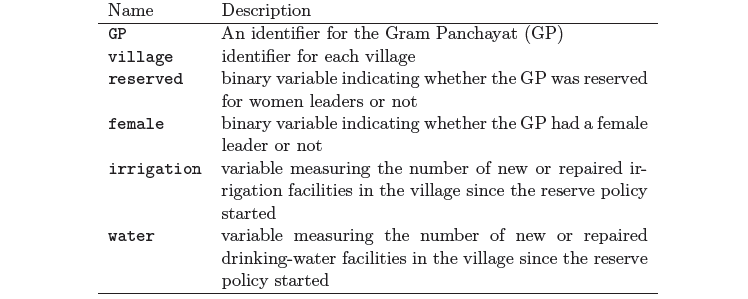
\includegraphics[width=1.1\textwidth]{women_desc.png}
\end{figure}		

\newpage
\begin{enumerate}
	\item [(a)] State a null and alternative (two-tailed) hypothesis. 
	\vspace{.5cm}
	
	Our model would be: 
	\begin{equation}
		y = a + bx
	\end{equation}
	Where: 
		\begin{itemize}
		\item x: policy (reserved / not reserved; I assume that 1 means reserved for women, 0 means not)
		\item y:  no. of new or repaired water facilities 
	\end{itemize}
	And so our hypotheses would be (we can hypothesize about effects because the presence of the policy in villages is random): 
	\begin{itemize}
		\item H0: The reservation policy has no effect on the no. of new/repaired water facilities.
		\item Ha: The policy does have an effect on the no. of new/repaired water facilities. 
	\end{itemize}
		
	\item [(b)] Run a bivariate regression to test this hypothesis in \texttt{R} (include your code!).
	\vspace{.5cm}
	
	\noindent \textbf {Code to run the regression:}
	\lstinputlisting[language=R, linerange={119-130}]{PS02_SC_Answers.R}
	
	\item [(c)] Interpret the coefficient estimate for reservation policy. 
	\vspace{.5cm}
	
	The coefficient estimate for reservation (b) is 9.25. It is positive, and it is quite sizable. This estimate indicates that, on average, places where the reservation policy is in place have 9.25 more new or repaired water facilities, as compared to villages where the policy is not in place. Therefore, the reservation policy does have an effect over the no. of new/repaired water facilities, and having government positions reserved for women does lead, in this case, to the implementation of more policies that women support. 
	
\end{enumerate}

\end{document}
